\chapter{有机金属化学：成键与配体}\label{ch:b3:organometallic-bonding}

1951 年，两个研究小组各自独立地得到了一种橙色、在空气中稳定的粉末，
其化学式为 $\ce{FeC10H10}$，这一结果令人费解：铁通常不会与碳形成稳定的键，
更不可能同时与两个环戊二烯基成键。
一年之内，其结构即已确定：铁原子位于两个平行的环之间，
与十个碳原子等同地成键，形成“三明治”结构。二茂铁
开启了现代有机金属化学，如今其催化剂生产了世界上大部分的聚合物、药物和精细化学品
（见\cref{ch:b3:homogeneous-catalysis}）。
本章讲述金属如何与一氧化碳、膦、烯烃、环状配体、卡宾以及金属之间
成键，以及等瓣类比如何将有机金属片段
与碳的有机化学联系起来。

\begin{recall}
本科一年级分册定义了有机金属化合物，并使用了格氏试剂。
本科二年级分册介绍了 18 电子规则和价电子计数、哈普托数、
$\pi$ 受体配体与 $\pi$ 给体配体（及其反馈键合），
以及有机金属反应的基元反应（氧化加成、还原消除、插入）
和片段轨道。\Cref{ch:b3:group-theory-applied} 统计了羰基的
红外活性 CO 伸缩振动，并构造了对称性匹配组合；
\cref{ch:b3:complex-spectra-magnetism} 将磁矩与
未成对电子联系起来。
\end{recall}

\begin{omfigure}
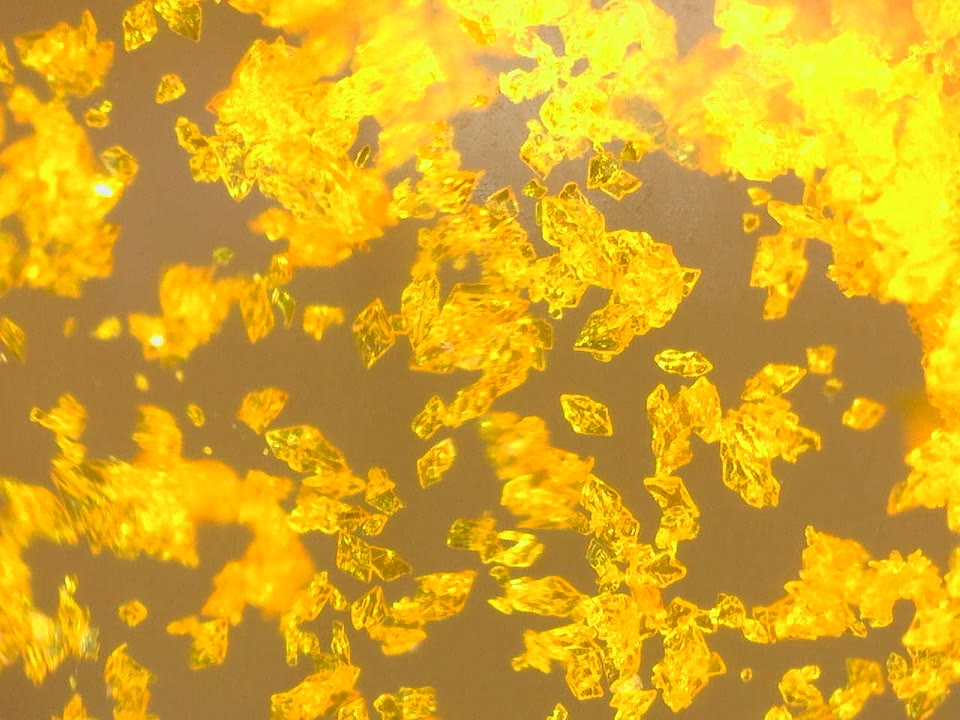
\includegraphics[width=0.5\linewidth]{images/book4/ferrocene-crystals.jpg}

{\small 二茂铁晶体，$\ce{Fe(C5H5)2}$：一种橙色的有机金属化合物，
在空气中稳定，微热即可升华。}
\end{omfigure}

\section{电子计数与氧化态}

\begin{method}[两种电子计数方法]\label{met:b3:organometallic-bonding:count}
\begin{enumerate}
  \item 中性配体（共价）法：金属提供其族数个电子；每个配体按中性计，
        提供 1 个（H、\ce{CH3}、Cl、$\eta^1$-烯丙基）或 2 个（CO、\ce{PR3}、烯烃）
        或更多个（$\eta^5$-\ce{C5H5} 为 5 个，$\eta^6$-\ce{C6H6} 为 6 个）电子；
        每个金属–金属键加 1 个，并对总电荷进行修正。
  \item 离子法：将 H、\ce{CH3}、Cl、\ce{C5H5} 等配体视为阴离子计数，
        分别提供 2、2、2 和 6 个电子；金属视为所生成的阳离子 $d^n$，
        中性配体的处理同前。
  \item 两种方法所得的总数相同；离子法还能给出氧化态
        和 $d^n$ 计数。
\end{enumerate}
\end{method}

\begin{example}[计数]\label{ex:b3:organometallic-bonding:count}
$\ce{Fe(CO)5}$：$8 + 5 \times 2 = 18$，铁（0 价），$d^8$。二茂铁：中性配体法 $8 + 2 \times 5 = 18$；离子法
$\ce{Fe^{2+}}$（$d^6$，6）$+ 2 \times 6$（$\ce{C5H5-}$）$= 18$，铁（II）。$\ce{Mn2(CO)10}$：每个 Mn 为 $7 + 5 \times 2 + 1$（Mn–Mn
键）$= 18$。方形平面 $d^8$ 配合物，如 $\ce{[PtCl4]^{2-}}$ 或威尔金森催化剂
$\ce{RhCl(PPh3)3}$，具有 16 个电子：其空的、类 $p_z$ 的轨道能级过高而无法被填充，
而 16 电子的方形平面配合物与 18 电子配合物同样稳定。
\end{example}

\section{羰基与膦}

\begin{definition}[金属羰基化合物]\label{def:b3:organometallic-bonding:carbonyl}
称\emph{金属羰基化合物}\index{金属羰基化合物}为以一氧化碳
为配体的配合物。\emph{端基羰基}\index{端基羰基}通过碳原子与
一个金属成键；\emph{桥联羰基}\index{桥联羰基}跨越两个（或三个）
金属。
\end{definition}

路德维希·蒙德于 1890 年发现，镍在常温下与一氧化碳反应，
生成易挥发的液体 $\ce{Ni(CO)4}$，该物质受热后又分解为纯镍，
这是一种精炼工艺的基础。一氧化碳通过其最高占据轨道与过渡金属成键，
该轨道为主要位于碳上的 $\sigma$ 孤对；同时，一氧化碳可将电子接受到
其空的 $\pi^*$ 轨道中，该轨道同样主要分布在
碳上。

\begin{definition}[协同成键]\label{def:b3:organometallic-bonding:synergic}
\emph{协同成键}\index{协同成键}指配体向金属的 $\sigma$ 给予与金属向配体的
$\pi$ 反馈键合相互增强：给予使金属上的电子更为丰富，
从而更易将电子反馈回去；
反馈键合则消除了因给予而积累的电荷。
\end{definition}

\begin{omfigure}
\begin{tikzpicture}[font=\small, >=Stealth]
  % sigma donation
  \fill[black!70] (0,0) circle (0.14); \node[anchor=north] at (0,-0.4) {M};
  \pic at (0,0) {omlobe={-0.7}{180}};
  \pic at (0,0) {omlobe={0.9}{0}};
  \node[circle, fill=black!40, inner sep=1.6pt] at (1.9,0) {};
  \node[circle, fill=omThm!70, inner sep=1.6pt] at (3.0,0) {};
  \pic at (1.9,0) {omlobe={0.85}{180}};
  \node[font=\scriptsize, anchor=north] at (1.9,-0.25) {C};
  \node[font=\scriptsize, anchor=north] at (3.0,-0.25) {O};
  \draw[->, thick, omThm] (1.4,0.55) to[bend right=30] (0.6,0.55);
  \node[anchor=north] at (1.5,-1.55) {$\sigma$ 给予};
  % pi back-donation
  \begin{scope}[xshift=6.0cm]
    \fill[black!70] (0,0) circle (0.14); \node[anchor=north] at (0,-1.1) {M};
    \pic at (0,0) {omdxz};
    \node[circle, fill=black!40, inner sep=1.6pt] at (1.9,0) {};
    \node[circle, fill=omThm!70, inner sep=1.6pt] at (3.0,0) {};
    \pic at (1.9,0) {omp={0.9}{90}};
    \pic at (3.0,0) {omp={-0.6}{90}};
    \draw[->, thick, omThm] (0.6,1.05) to[bend left=30] (1.6,1.05);
    \node[anchor=north] at (1.5,-1.55) {$\pi$ 反馈键合};
  \end{scope}
\end{tikzpicture}

{\small 一氧化碳的协同成键。左：碳上的孤对（$\sigma$
轨道）给予一个空的 $\sigma$ 型金属轨道。右：一个充满电子的金属 $d$
轨道（$d_{xz}$，沿两个坐标轴）与 CO 的空 $\pi^*$ 轨道发生重叠，该轨道在碳上的贡献较大，
其瓣的相位与之相匹配：电子回流到一个
在 C 与 O 之间具有反键性质的轨道中。}
\end{omfigure}

\begin{proposition}[CO 伸缩波数]\label{prop:b3:organometallic-bonding:co-frequency}
金属对 CO 配体的 $\pi^*$ 轨道反馈键合越强，
C--O 伸缩波数就越低。
\end{proposition}

\begin{proof}[论证]
CO 的 $\pi^*$ 轨道在 C 与 O 之间具有反键性质：占据它们会削弱
C--O 键，降低其力常数，从而降低伸缩波数，
而波数与力常数的平方根成正比（见\cref{ch:b3:rovibrational-spectroscopy}）。
$\sigma$ 给予会使电子从一个对 C--O 而言几乎非键
（略具反键性）的轨道中移出，单独来看会使波数略有升高：
但观测到的下降表明反馈键合占主导。
\end{proof}

游离一氧化碳的基频为 $\omega_e - 2\omega_ex_e = \qty{2143}{cm^{-1}}$；端基
羰基在中性配合物中大致吸收于 1900 至 \qty{2100}{cm^{-1}} 之间，
桥联羰基的吸收更低。在等电子系列中，阴离子
羰基的吸收波数低于中性者，阳离子者则
在更高处吸收：金属越富电子，反馈键合越强。谱带数
目可由对称性（见\cref{ch:b3:group-theory-applied}）确定构型。
% ledger: diat:CO.we, diat:CO.wexe

\begin{proposition}[$\pi$ 相互作用与配体场分裂]\label{prop:b3:organometallic-bonding:pi-delta}
在八面体配合物中，$\pi$ 受体配体使 $\Delta_{\mathrm o}$ 增大，$\pi$ 给体配体
则使其减小。
\end{proposition}

\begin{proof}
$e_g$ 轨道仅具有 $\sigma$ 对称性。$t_{2g}$ 轨道（$d_{xy}$、$d_{xz}$、$d_{yz}$）与一个 $t_{2g}$
组合相匹配，该组合由配体的 $\pi$ 轨道构成：对 $d_{xy}$ 而言，$xy$ 平面内的四个配体各
提供一个在该平面内垂直于其 M--L 轴的 $\pi$ 轨道，而
符号交替的组合具有 $d_{xy}$ 的对称性（其余
组合按 $t_{1g}$、$t_{1u}$ 和 $t_{2u}$ 变换，与 $d$ 轨道无对应）。两个
同对称性的轨道会混合并相互排斥：较低者被压低，较高者被抬高。一个
$\pi$ 受体在 $t_{2g}$ 组之上提供空轨道，使该组被压低，$\Delta_{\mathrm o}$
增大。$\pi$ 给体在其下方提供已填充轨道，使之被抬高，$\Delta_{\mathrm o}$
减小。两种情形下，$e_g$ 能级均不受影响。
\end{proof}

这就是为何 CO 和 \ce{CN-} 位于光谱化学序列的强端，
而卤化物与氢氧化物位于弱端，正如本科二年级分册所述。

\begin{definition}[托尔曼参数]\label{def:b3:organometallic-bonding:tolman}
膦的\emph{托尔曼锥角}\index{托尔曼锥角}是一个锥体的顶角，该锥体以金属为中心，
位于标准距离处，恰好包住其取代基的范德瓦耳斯表面，
是衡量膦大小的量度。
\emph{托尔曼电子参数}\index{托尔曼电子参数}是
$\ce{Ni(CO)3L}$ 中对称 CO 伸缩振动的波数：膦 L 给电子越强，
该波数越低。
\end{definition}

膦的大小与给电子能力可分别通过取代基调节：
三烷基膦的给电子能力强于三芳基膦，
亚磷酸酯最弱；$\ce{P(tBu)3}$ 远比 $\ce{PMe3}$ 庞大。大体积膦有利于
形成较低的配位数并使配体快速解离，这正是它们
大量见于各类催化剂中。

\section{$\pi$ 配体}

\begin{definition}[杜瓦–查特–邓肯森模型]\label{def:b3:organometallic-bonding:dcd}
\emph{杜瓦–查特–邓肯森模型}\index{杜瓦–查特–邓肯森模型}描述烯烃与金属
的成键，它结合了 $\sigma$ 给予（由 C=C $\pi$ 轨道流向金属空轨道）与
由充满电子的金属 $d$ 轨道
向 C=C $\pi^*$ 轨道的反馈键合。其强反馈极限是
\emph{金属环丙烷}\index{金属环丙烷}，即一个三元环，
含两个 M--C $\sigma$ 键与一个 C--C 单键。
\end{definition}

\begin{proposition}[向烯烃反馈键合的后果]\label{prop:b3:organometallic-bonding:dcd}
配位使 C=C 键变长，并使取代基向远离
金属的方向弯折，且反馈键合越强，弯折越明显。
\end{proposition}

\begin{proof}[论证]
将电子从 $\pi$（成键）轨道移出并加入 $\pi^*$
（反键）轨道，两者都会降低 C--C 键级。混入 $\pi^*$ 成分
使碳原子向 $sp^3$ 重新杂化，其与取代基的键
朝远离金属的方向伸展，趋向金属环丙烷的几何构型。
\end{proof}

\begin{omfigure}
\begin{tikzpicture}[font=\small, >=Stealth]
  \fill[black!70] (0,0) circle (0.14); \node[anchor=north] at (0,-1.1) {M};
  \pic at (0,0) {omlobe={0.9}{0}};
  \foreach \y in {0.45,-0.45}{\node[circle, fill=black!40, inner sep=1.6pt] at (1.9,\y) {};}
  \pic at (1.9,0.45) {omp={-0.75}{0}};
  \pic at (1.9,-0.45) {omp={-0.75}{0}};
  \draw[->, thick, omThm] (1.3,1.0) to[bend right=30] (0.5,0.6);
  \node[anchor=north] at (1.2,-1.4) {$\sigma$: $\pi$(C=C) $\to$ M};
  \begin{scope}[xshift=5.6cm]
    \fill[black!70] (0,0) circle (0.14); \node[anchor=north] at (0,-1.1) {M};
    \pic at (0,0) {omdxy};
    \foreach \y in {0.45,-0.45}{\node[circle, fill=black!40, inner sep=1.6pt] at (1.9,\y) {};}
    \pic at (1.9,0.45) {omp={-0.75}{0}};
    \pic at (1.9,-0.45) {omp={0.75}{0}};
    \draw[->, thick, omThm] (0.7,0.9) to[bend left=30] (1.5,0.9);
    \node[anchor=north] at (1.2,-1.4) {$\pi$: M $\to$ $\pi^*$(C=C)};
  \end{scope}
\end{tikzpicture}

{\small 侧位配位烯烃的杜瓦–查特–邓肯森模型（
C=C 竖直，金属在左侧）。左：充满电子的 $\pi$ 轨道（两个 $p$ 轨道
同相）向空的金属轨道给予电子。右：充满电子的金属 $d$ 轨道
相位匹配，向空的 $\pi^*$ 轨道给予电子（两个 $p$ 轨道
反相）。}
\end{omfigure}

蔡斯盐 $\ce{K[PtCl3(C2H4)]}$ 于 1827 年制得，是首个
过渡金属的有机金属化合物；其乙烯垂直于 \ce{PtCl3} 平面，
与该模型的预言一致。烯丙基（$\eta^3$）、二烯（$\eta^4$）、芳烃（$\eta^6$）以及环戊二烯基
环（$\eta^5$）以相同方式通过多个碳原子同时配位。

\begin{definition}[茂金属]\label{def:b3:organometallic-bonding:metallocene}
称\emph{夹心化合物}\index{夹心化合物}为金属位于两个平行平面环配体之间、
且通过环上全部碳原子与金属成键的化合物；\emph{茂金属}\index{茂金属}为
带有两个 $\eta^5$-环戊二烯基环的夹心化合物，
即 $\ce{M(C5H5)2}$。
\end{definition}

\begin{proposition}[二茂铁的前线轨道]\label{prop:b3:organometallic-bonding:ferrocene}
在具有平行环（$D_{5d}$）的茂金属中，金属的 $d$ 轨道分裂为 $e_{2g}$
（$d_{xy}$、$d_{x^2-y^2}$）和 $a_{1g}$（$d_{z^2}$），近似非键且能级接近，以及 $e_{1g}^\ast$（$d_{xz}$、
$d_{yz}$）为强反键轨道；二茂铁中六个 $d$ 电子占据 $e_{2g}^4a_{1g}^2$，总计 18
个电子，且无未成对电子。
\end{proposition}

\begin{proof}[论证]
两个环的 $\pi$ 轨道组合成对称性匹配组合 $a_{1g}$、$a_{2u}$、
$e_{1g}$、$e_{1u}$、$e_{2g}$、$e_{2u}$（由每个环的五个 $\pi$ 轨道得到，沿轴分别有零、一、二个节面）。
充满电子的环 $e_{1g}$ 组合与 $d_{xz}$、$d_{yz}$（各沿轴含一个节面）强烈重叠，
形成以环为主的成键轨道，以及以金属为主、能级被推高的反键 $e_{1g}^\ast$。
$d_{xy}$、$d_{x^2-y^2}$（两个节面）只与空的环 $e_{2g}$ 轨道作用，
经反馈键合略有稳定化；
$d_{z^2}$ 指向每个环中心的空穴，几乎不重叠。
六个电子填充 $e_{2g}$ 与 $a_{1g}$；
加上成键环组合中的十二个电子，总数为 18。
\end{proof}

\begin{omfigure}
\begin{tikzpicture}[font=\small]
  % sandwich drawing
  \begin{scope}[xshift=-1.0cm]
    \draw[thick, fill=black!8] (0,1.0) ellipse (1.0 and 0.3);
    \draw[thick, fill=black!8] (0,-1.0) ellipse (1.0 and 0.3);
    \foreach \a in {90,162,234,306,18}{\fill[black!60] ({cos(\a)},{1.0+0.3*sin(\a)}) circle (0.07);
      \fill[black!60] ({cos(\a)},{-1.0+0.3*sin(\a)}) circle (0.07);}
    \shade[ball color=orange!70!brown] (0,0) circle (0.2);
    \node[anchor=west] at (0.25,0) {Fe};
  \end{scope}
  % level diagram for four metallocenes
  \pic[transform shape] at (2.1,-0.9) {omlevel={u}{0.5}};
  \pic[transform shape] at (2.7,-0.9) {omlevel={ud}{0.5}};
  \pic[transform shape] at (2.4,-0.4) {omlevel={ud}{0.5}};
  \pic[transform shape] at (2.1,1.0) {omlevel={}{0.5}};
  \pic[transform shape] at (2.7,1.0) {omlevel={}{0.5}};
  \node[anchor=north] at (2.4,-1.3) {二茂铁阳离子 \ce{[FeCp2]+}};
  \node[anchor=north, font=\scriptsize] at (2.4,-1.75) {17 e$^-$};
  \pic[transform shape] at (4.3,-0.9) {omlevel={ud}{0.5}};
  \pic[transform shape] at (4.9,-0.9) {omlevel={ud}{0.5}};
  \pic[transform shape] at (4.6,-0.4) {omlevel={ud}{0.5}};
  \pic[transform shape] at (4.3,1.0) {omlevel={}{0.5}};
  \pic[transform shape] at (4.9,1.0) {omlevel={}{0.5}};
  \node[anchor=north] at (4.6,-1.3) {二茂铁 \ce{FeCp2}};
  \node[anchor=north, font=\scriptsize] at (4.6,-1.75) {18 e$^-$};
  \pic[transform shape] at (6.5,-0.9) {omlevel={ud}{0.5}};
  \pic[transform shape] at (7.1,-0.9) {omlevel={ud}{0.5}};
  \pic[transform shape] at (6.8,-0.4) {omlevel={ud}{0.5}};
  \pic[transform shape] at (6.5,1.0) {omlevel={u}{0.5}};
  \pic[transform shape] at (7.1,1.0) {omlevel={}{0.5}};
  \node[anchor=north] at (6.8,-1.3) {二茂钴 \ce{CoCp2}};
  \node[anchor=north, font=\scriptsize] at (6.8,-1.75) {19 e$^-$};
  \pic[transform shape] at (8.7,-0.9) {omlevel={ud}{0.5}};
  \pic[transform shape] at (9.3,-0.9) {omlevel={ud}{0.5}};
  \pic[transform shape] at (9.0,-0.4) {omlevel={ud}{0.5}};
  \pic[transform shape] at (8.7,1.0) {omlevel={u}{0.5}};
  \pic[transform shape] at (9.3,1.0) {omlevel={u}{0.5}};
  \node[anchor=north] at (9.0,-1.3) {二茂镍 \ce{NiCp2}};
  \node[anchor=north, font=\scriptsize] at (9.0,-1.75) {20 e$^-$};
  \node[anchor=east, font=\scriptsize] at (1.8,-0.9) {$e_{2g}$};
  \node[anchor=east, font=\scriptsize] at (1.8,-0.4) {$a_{1g}$};
  \node[anchor=east, font=\scriptsize] at (1.8,1.0) {$e_{1g}^\ast$};
\end{tikzpicture}

{\small 左：二茂铁的夹心结构（重叠式环）。右：茂金属以 $d$ 轨道为主的前线轨道，
$e_{2g}$ 与 $a_{1g}$ 近似非键，$e_{1g}^\ast$ 为反键，
这些轨道分别在二茂铁阳离子（17 个电子）、二茂铁（18 个）、
二茂钴（19 个）和二茂镍（20 个，每个 $e_{1g}^\ast$ 轨道各有一个电子，
按洪特规则自旋平行）中被填充。}
\end{omfigure}

\section{卡宾、卡拜与金属–金属键}

\begin{definition}[卡宾与卡宾配合物]\label{def:b3:organometallic-bonding:carbene}
称 $\ce{R2C}$ 为\emph{卡宾}\index{卡宾}，
它是中性物种，二价碳原子上带有两个非键电子。称\emph{卡宾配合物}\index{卡宾配合物}
为含 $\ce{CR2}$ 配体、通过双键与金属相连（即 $\ce{M=CR2}$）的配合物。
\emph{费歇尔卡宾}\index{费歇尔卡宾}配合物的卡宾碳上
连有杂原子取代基，金属为低价态并带有 $\pi$ 受体配体，
其卡宾碳具有亲电性。
\emph{施罗克卡宾}\index{施罗克卡宾}（亚烷基）配合物仅带 C 或 H 取代基，
金属为高价态的前过渡金属，其碳具有亲核性。
\emph{氮杂环卡宾}\index{氮杂环卡宾}是两侧各连有一个氮原子的环状卡宾，
可作为自由化合物稳定存在，是强的 $\sigma$ 给体配体。
\end{definition}

两类卡宾配合物的差别在于 M=C 键的共享方式。
在费歇尔卡宾中，单重态卡宾将其孤电子对给予金属，同时接受金属的反馈键合，
电子进入其空的 $p$ 轨道；杂原子的孤电子对也起稳定作用，
因此碳仍然缺电子，易受亲核试剂进攻。在施罗克卡宾中，金属与卡宾两个三重态片段
形成共价的 $\sigma +
\pi$ 键，电子偏向碳一侧，亚烷基的行为与维蒂希叶立德相似。

\begin{definition}[卡拜配合物]\label{def:b3:organometallic-bonding:carbyne}
称\emph{卡拜配合物}\index{卡拜配合物}为金属与带一个取代基的碳原子之间
形成三键的配合物，即 $\ce{M#CR}$。
\end{definition}

\begin{definition}[$\delta$ 键、四重键]\label{def:b3:organometallic-bonding:delta}
称轨道具有两个包含核间轴的节面的键为\emph{$\delta$ 键}\index{$\delta$ 键}，
它由两个 $d$ 轨道（如 $d_{xy}$ 与 $d_{xy}$）面对面重叠形成。
由一个 $\sigma$ 键、两个 $\pi$ 键和一个 $\delta$ 键在两个金属原子之间构成的键，
称为\emph{四重键}\index{四重键}。
\end{definition}

\begin{proposition}[{$[\mathrm{Re_2Cl_8}]^{2-}$ 的四重键}]\label{prop:b3:organometallic-bonding:quadruple}
在 $\ce{[Re2Cl8]^{2-}}$ 中（两个 \ce{Re^{III}}，各为 $d^4$），八个 $d$ 电子占据 $\sigma^2\pi^4\delta^2$，
即键级为 4，这要求两个 \ce{ReCl4} 单元呈重叠式构象。
\end{proposition}

\begin{proof}
取 $z$ 沿 Re--Re 轴，每个 Re 上的 Cl 原子沿 $\pm x$ 与 $\pm y$ 方向，
$d_{x^2-y^2}$ 指向氯原子，并参与 Re--Cl 成键。其余四个 $d$ 轨道
在每个金属上两两重叠：$d_{z^2}$ 与 $d_{z^2}$ 沿轴重叠（$\sigma$），$d_{xz}$ 与 $d_{xz}$ 以及
$d_{yz}$ 与 $d_{yz}$ 并排重叠（$\pi$，共两次），$d_{xy}$ 与 $d_{xy}$ 面对面重叠（$\delta$，最弱）。
八个电子填满四个成键组合。将一个单元旋转 $45^\circ$（绕 $z$ 轴），
其 $d_{xy}$ 变为 $d_{x^2-y^2}$，由于对称性，它与另一个 $d_{xy}$ 的重叠为零：
$\delta$ 键，连同重叠式构象的偏好，随之消失。其
余三种重叠具有柱对称性，或大小不变。
\end{proof}

% ledger: geom:Re2Cl8.ReRe
钾盐中 Re--Re 距离为 \qty{2.24}{\angstrom}，对两个金属原子而言很短，
两半的氯配体确实呈重叠式构象，尽管存在空间排斥：$\delta$ 键虽弱，却将它们保持在此构型中。

\begin{omfigure}
\tdplotsetmaincoords{58}{25}
\begin{tikzpicture}[tdplot_main_coords, font=\small, scale=1.15]
  \draw[thick, black!60] (0,0,0) -- (0,0,2.0);
  \foreach \z in {0,2.0}{
    \foreach \b in {0,90,180,270}{
      \draw[black!45] (0,0,\z) -- ({1.55*cos(\b)},{1.55*sin(\b)},\z);}
    \foreach \a/\s in {45/omphasepos, 135/omphaseneg, 225/omphasepos, 315/omphaseneg}{
      \path[\s, opacity=0.9] plot[domain=0:360, samples=48, smooth cycle]
        ({0.62*cos(\a)+0.55*cos(\x)*cos(\a)-0.26*sin(\x)*sin(\a)},
         {0.62*sin(\a)+0.55*cos(\x)*sin(\a)+0.26*sin(\x)*cos(\a)}, {\z});}
    \foreach \b in {0,90,180,270}{
      \node[circle, fill=green!45!black, inner sep=1.8pt] at ({1.55*cos(\b)},{1.55*sin(\b)},\z) {};}
    \shade[ball color=black!40] (0,0,\z) circle (0.14);}
  \node[anchor=east, xshift=-1.9cm] at (0,0,2.0) {Re};
  \node[anchor=east, xshift=-1.9cm] at (0,0,0) {Re};
\end{tikzpicture}

{\small $\delta$ 分量属于 $\ce{[Re2Cl8]^{2-}}$ 的四重键：两个铼原子的 $d_{xy}$ 轨道
（各四瓣，正负号分别以蓝色与橙色表示）沿 Re--Re 轴面对面相对，
同号瓣相对。氯原子（绿色）
呈重叠式构象，位于 $x$ 与 $y$ 方向上、瓣与瓣之间。}
\end{omfigure}

\section{等瓣类比}

\begin{definition}[等瓣片段]\label{def:b3:organometallic-bonding:isolobal}
若两个分子片段的
前线轨道数、对称性、近似能量和形状，以及其中的电子数均相近，则称二者为\emph{等瓣的}\index{等瓣的}。
\emph{等瓣类比}\index{等瓣类比}预言，
等瓣片段可以在分子中
相互替换。
\end{definition}

\begin{proposition}[等瓣系列]\label{prop:b3:organometallic-bonding:isolobal}
$\ce{CH3}$、$\ce{Mn(CO)5}$ 与 $\ce{CpFe(CO)2}$ 互为等瓣的（一个前线轨道，一个电子）；
$\ce{CH2}$ 与 $\ce{Fe(CO)4}$（两个轨道、两个电子）；$\ce{CH}$ 与 $\ce{Co(CO)3}$（三个轨道，
三个电子）。
\end{proposition}

\begin{proof}[论证]
$\ce{CH3}$ 是缺少一个键的四面体片段，具有一个类 $sp^3$ 的轨道和一个电子，
比八电子结构少一个电子。$\ce{Mn(CO)5}$ 是缺少一个配体的八面体，其
空位上有一个指向外侧的杂化轨道；$7 + 10 = 17$ 个电子，比 18 少一个，
其单电子位于该杂化轨道中。移去两个或三个
配体（或键）则分别得到两个或三个这样的轨道与电子，两侧
的计数方式相同：$\ce{Fe(CO)4}$ 有 16 个电子（$8 + 8$），比 18 少两个；
$\ce{Co(CO)3}$ 有 15 个电子（$9 + 6$），少三个。
\end{proof}

\begin{method}[通过等瓣替换预测结构]\label{met:b3:organometallic-bonding:isolobal}
\begin{enumerate}
  \item 将化合物拆分为片段，
        数出每个片段的前线轨道与电子数。
  \item 将每个片段替换为其有机等瓣对应物。
  \item 若存在对应的有机类似物，可由其推断成键方式与分子形状：
        $\ce{Mn2(CO)10}$ 相当于“乙烷”，$\ce{Co3(CO)9CH}$ 相当于“四面体烷” $\ce{(CH)4}$，其中三个 CH
        被 $\ce{Co(CO)3}$ 取代。
\end{enumerate}
\end{method}

\begin{omfigure}
\begin{tikzpicture}[font=\small]
  \foreach \y/\l/\r/\n in {0/{\ce{CH3}}/{\ce{Mn(CO)5}}/1, -1.6/{\ce{CH2}}/{\ce{Fe(CO)4}}/2, -3.2/{\ce{CH}}/{\ce{Co(CO)3}}/3}{
    \node at (0,\y) {\l};
    \node at (5.2,\y) {\r};
    \node[font=\large] at (2.6,\y) {$\longleftrightarrow$};
    \node[font=\scriptsize, anchor=south] at (2.6,\y+0.15) {等瓣};
    \node[font=\scriptsize, anchor=west] at (7.0,\y) {\ifnum\n=1 一个前线轨道，一个电子\else\ifnum\n=2 两个前线轨道，两个电子\else 三个前线轨道，三个电子\fi\fi};}
  \foreach \a in {0}{\pic at (0.55,0) {omlobe={0.6}{0}};}
  \pic at (6.25,0) {omlobe={0.6}{0}};
  \pic at (0.45,-1.6) {omlobe={0.6}{20}}; \pic at (0.45,-1.6) {omlobe={0.6}{-20}};
  \pic at (6.15,-1.6) {omlobe={0.6}{20}}; \pic at (6.15,-1.6) {omlobe={0.6}{-20}};
  \foreach \t in {-30,0,30}{\pic at (0.4,-3.2) {omlobe={0.55}{\t}}; \pic at (6.1,-3.2) {omlobe={0.55}{\t}};}
\end{tikzpicture}

{\small 等瓣系列（前线杂化轨道为示意）：每个有机片段与其对面的
金属羰基片段，朝外指向的前线轨道数相同，
其中的电子数也相同，
并以类似方式结合。}
\end{omfigure}

\begin{definition}[抓氢相互作用]\label{def:b3:organometallic-bonding:agostic}
\emph{抓氢相互作用}\index{抓氢相互作用}是金属与其自身配体的一条 C--H 键之间
形成的三中心二电子键，
其中 C--H 成键电子对向金属的空轨道提供电子。
\end{definition}

抓氢原子在衍射结构中表现为金属与氢原子的距离较短，
C--H 伸缩振动波数异常低，并在核磁共振谱中表现为
化学位移移向高场，$^1J_{\mathrm{CH}}$ 耦合常数减小。它们是 C--H 活化的
冻结快照，而 C--H 活化是许多催化反应的第一步。

\begin{inthelab}[金属羰基化合物的操作]
金属羰基化合物应在通风橱中操作，通风橱须正常排风，并在氮气或氩气保护下进行，
且禁止明火：许多羰基化合物受热时会释放一氧化碳。
挥发性羰基化合物应使用套管转移，或在真空线上操作，切勿倾倒；
残液应在通风橱中以缓慢氧化的方式销毁（使用漂白水或溴水）。
毒性最大的四羰基合镍，
在教学实验室中根本不予使用。
\end{inthelab}

\begin{safety}{\ghs[0.62cm]{GHS02}\ghs[0.62cm]{GHS06}\ghs[0.62cm]{GHS07}\ghs[0.62cm]{GHS08}\ghs[0.62cm]{GHS09}}
% ledger: ghs4:NiCO4, ghs4:ferrocene
四羰基合镍：高度易燃，吸入致命，疑似致癌物，
可能损害胎儿。二茂铁：易燃固体，吞食有害；
作为精细化学品处理，操作时戴手套并防止粉尘。
\end{safety}

\begin{history}[蒙德的羰基化合物与夹心结构]
路德维希·蒙德及其同事于 1890 年发现四羰基合镍，
当时正研究一氧化碳对镍阀门的腐蚀，并在此基础上建立了镍的精炼工艺。
二茂铁于 1951 年由托马斯·凯利和彼得·
保森制得，并由塞缪尔·米勒、约翰·特博思和约翰·特雷梅因独立制得；1952 年，
杰弗里·威尔金森、罗伯特·伍德沃德和恩斯特·奥托·费歇尔提出了
夹心结构。费歇尔与威尔金森共同获得 1973 年诺贝尔
化学奖，表彰二人在夹心化合物方面的工作。
\end{history}

\section{练习}

\begin{exercise}[$\star$]\label{exo:b3:organometallic-bonding:1}
计算下列物种的价电子数：$\ce{Fe(CO)5}$、$\ce{Mn2(CO)10}$（按每个 Mn 计）、$\ce{CpMo(CO)3H}$、蔡斯阴离子
$\ce{[PtCl3(C2H4)]-}$、$\ce{Cr($\eta^6$-C6H6)(CO)3}$ 和 $\ce{Cp2ZrCl2}$。
\end{exercise}

\begin{exercise}[$\star$]\label{exo:b3:organometallic-bonding:2}
给出上一题中各化合物里金属的氧化态和
$d^n$ 电子数。
\end{exercise}

\begin{exercise}[$\star$]\label{exo:b3:organometallic-bonding:3}
比较 $\ce{[V(CO)6]-}$、$\ce{Cr(CO)6}$ 和 $\ce{[Mn(CO)6]+}$ 的 CO 伸缩振动波数的大小顺序，并说明理由。
\end{exercise}

\begin{exercise}[$\star$]\label{exo:b3:organometallic-bonding:4}
给出 $\ce{Mn2(CO)10}$、$\ce{[CpFe(CO)2]2}$ 和 $\ce{Co3(CO)9CH}$ 的有机等瓣类似物。
\end{exercise}

\begin{exercise}[$\star\star$]\label{exo:b3:organometallic-bonding:5}
$面式$-与 $经式$-$\ce{M(CO)3L3}$ 在红外光谱中各出现几条 CO 伸缩振动谱带？
\end{exercise}

\begin{exercise}[$\star\star$]\label{exo:b3:organometallic-bonding:6}
解释在催化剂中将 $\ce{PMe3}$ 换成 $\ce{P(tBu)3}$，为何能加快
一个需要配体从金属上离去的步骤。
\end{exercise}

\begin{exercise}[$\star\star$]\label{exo:b3:organometallic-bonding:7}
将 $\ce{(CO)5Cr=C(OMe)Ph}$ 和 $\ce{Ta(=CHCMe3)(CH2CMe3)3}$ 分别归类为费歇尔卡宾配合物或施罗克卡宾
配合物，并预测它们与胺和酮的反应。
\end{exercise}

\begin{exercise}[$\star\star$]\label{exo:b3:organometallic-bonding:8}
交叉式构象的 $\ce{[Re2Cl8]^{2-}}$ 其键级应为多少？
多了两个电子的 $\ce{[Re2Cl8]^{4-}}$，其键级是多少？
\end{exercise}

\begin{exercise}[$\star\star$]\label{exo:b3:organometallic-bonding:9}
列出支持存在抓氢 C--H 相互作用的三类证据。
\end{exercise}

\begin{exercise}[$\star\star\star$]\label{exo:b3:organometallic-bonding:10}
举出价电子数分别为 16、17 和 19 的稳定配合物的例子，并
解释每一种对 18 电子规则的例外。
\end{exercise}

\begin{exercise}[$\star\star\star$]\label{exo:b3:organometallic-bonding:11}
$\ce{Cr(CO)6}$ 无色且具有抗磁性。试利用 $\pi$ 受体效应对 $\Delta_{\mathrm o}$ 的影响，
解释其为何是低自旋，以及其 $d$--$d$ 谱带为何位于紫外区。
\end{exercise}

\begin{exercise}[$\star\star\star$]\label{exo:b3:organometallic-bonding:12}
乙烯的 C--C 键在蔡斯盐中由 \qty{1.34}{\angstrom} 伸长到 \qty{1.37}{\angstrom}，
在具有强反馈键合的低价金属配合物中伸长至约 \qty{1.43}{\angstrom}（数据
见本题）。试用杜瓦–查特–邓肯森模型解释。
\end{exercise}

\section{问题：夹心化合物}

\begin{problem}[{周末问题——夹心化合物：四种茂金属的电子计数、
前线轨道与未成对电子、氧化还原化学，以及两个
等瓣类比与光谱问题}]
\label{pb:b3:organometallic-bonding:1}
茂金属 $\ce{MCp2}$（$\ce{Cp} = \eta^5$-$\ce{C5H5}$）已知 M 为 Fe、Co、Ni 的情形，以及二茂铁阳离子。

\medskip\noindent\textbf{第一部分——计数。}
\begin{enumerate}
  \item 用离子法计算二茂铁的电子数。
  \item 用中性法计算其电子数。
  \item 计算钴茂的电子数。
  \item 计算镍茂的电子数。
  \item 计算二茂铁阳离子的电子数。
  \item 给出每种金属的氧化态和 $d^n$ 电子数。
\end{enumerate}

\medskip\noindent\textbf{第二部分——轨道与磁性。}
\begin{enumerate}[resume]
  \item 对五个 $d$ 轨道进行分类，所属点群为 $D_{5d}$。
  \item 其中哪些与环的 $\pi$ 轨道有强烈重叠，
        并会产生什么后果？
  \item 给出以 $d$ 轨道为基础的能级顺序。
  \item 填充二茂铁的这些轨道：未成对电子数是多少？
  \item 填充钴茂的这些轨道：未成对电子数及唯自旋磁矩是多少？
  \item 填充镍茂的这些轨道：未成对电子数及唯自旋磁矩是多少？
  \item 填充二茂铁阳离子的这些轨道：未成对电子数是多少？为何其实测磁矩
        高于唯自旋值？
\end{enumerate}

\medskip\noindent\textbf{第三部分——氧化还原。}
\begin{enumerate}[resume]
  \item 为何钴茂是一种强还原剂？
  \item 为何二茂铁/二茂铁阳离子电对的反应快且可逆？
  \item 为何它在非水电化学中被用作内参比，
        （见\cref{ch:b3:electrode-kinetics}）？
  \item 对镍茂与双电子配体的反应，你预期会
        有怎样的表现？
\end{enumerate}

\medskip\noindent\textbf{第四部分——片段与光谱。}
\begin{enumerate}[resume]
  \item 证明 $\ce{CpFe(CO)2}$ 与 \ce{CH3} 是等瓣的，并预测
        $\ce{[CpFe(CO)2]2}$ 的结构。
  \item 它与 $\ce{Mn(CO)5}$ 可能形成怎样的混合二聚体？
  \item 将 $\ce{CpMn(CO)3}$ 中的一个 CO 换成 $\ce{PPh3}$，其余
        CO 伸缩振动将如何变化？
  \item $\ce{Cr($\eta^6$-C6H6)(CO)3}$（$C_{3v}$）会出现几条 CO 谱带？
  \item 为何在取代过程中，$\eta^5$-Cp 环可以滑移为 $\eta^3$？
  \item 给出结果：镍茂的唯自旋磁矩。
\end{enumerate}
\end{problem}
